\section{Solving Identification with a Selection Model}
\label{sec:selectionmodel}
If your goal is to estimate CM effects, and you could control for unobserved selection terms $U_{0,i}, U_{1,i}$, then you would.
This ideal example would yield unbiased estimates.
% Alas, $U_i$ is by definition unobserved.
The selection model takes this insight seriously, providing conditions to model the implied unobserved confounding by $U_{0,i}, U_{1,i}$, and then control for it.

Writing here about how a \cite{heckman1974shadow} selection model purges selection bias.



Control function assumption + instrument.

Lemma: Under assumptions CF(1, 2, 3), mean POs are identified in the way written in Kline Walters (2019).
Needs an appendix proof.

And similarly for compiler POs.

=> direct and indirect effects are identified by a selection model.

4. Estimation with a Selection Model.

Go through the steps of a Heckman selection model,  and the corresponding SEs + reference n^0.5 consistency.

Reference an alternative to the functional form is using splines.  And reference Powell Newey for n^0.5 consistency, and normality.  This bootstrapped SEs.  Cross-fit to improve efficiency.

5. Simulation evidence.

Through all I have already put together.

FIrst paragraph on the general idea of using a selection model.  Include the E[Y | Z, D, X] version of the regression equation.
The key idea is using a selection model to nullify the error term in (1 - D) E[U_0 | D = 0] + D E[U_1 | D = 1] .  This is exploiting ideas from selection models + marginal TEs to identify this system, including using the selection model to identify the mediator compilers’ effect.  Indeed, mediation estimates already do a two-step procedure; it is a minor adjustment to include a CF  in the second-stage, to guard against selection-on-gains (chief among which is the Roy model).

Monotonicity gives selection model representation, D = 1{ \phi(Z, X) > V } which can be transformed into D = 1{ \pi(Z, X) > U } for U_i = F_V(V_i) ~ unif(0, 1).
CF assumption connects first-stage and second-stage errors, by assuming that Cov(U_i, U_1),Cov(U_i, U_0)  > 0.
Instrument separately identifies the propensity score (not technically required but needed for efficiency).

Under these assumptions, outcome regression has the following form.
E[Y | Z, D, X] = … + \rho_0 \lamda_0( \pi(Z_i, X_i)) + \rho_1 \lamda_1( \pi(Z_i, X_i))

Where \lambda_0, \lambda_1 are the control functions. For J(u) = F^-1_V(u) - E[ F^-1_V(U_i) ]

This is a special case of Heckman (1980), notation from Kiline Walters (2019).

\begin{figure}[h!]
    \caption{Simulated Distribution of CM Effect Estimates.}
    \begin{subfigure}[c]{0.475\textwidth}
        \centering
        \caption{ADE.}
        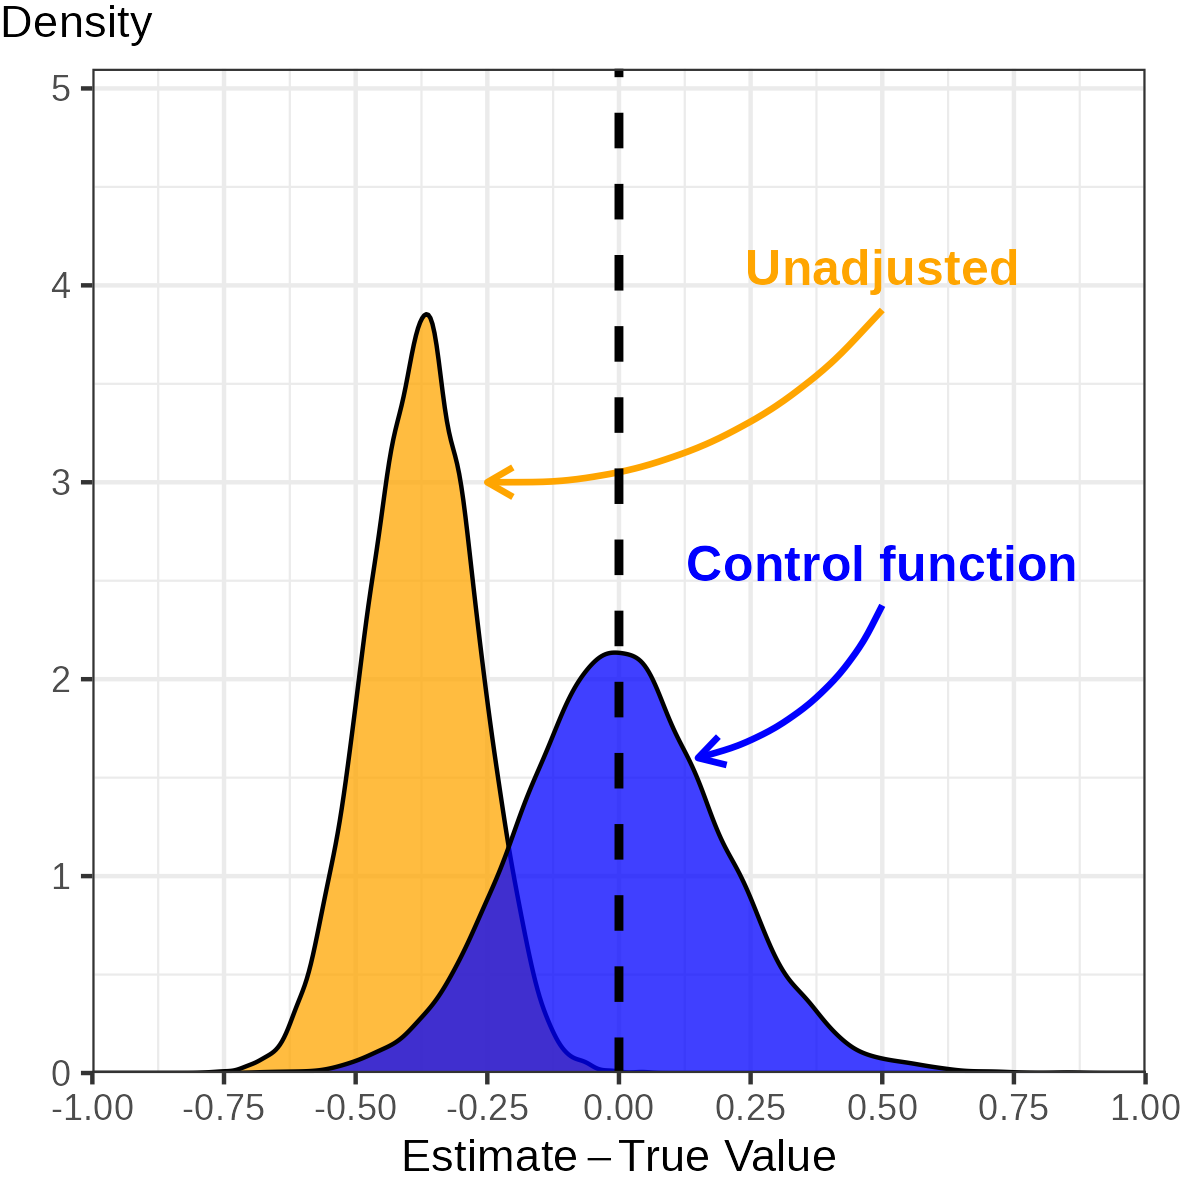
\includegraphics[width=\textwidth]{
            ../programs/simulations/sim-output/heckit-direct-dist.png}
    \end{subfigure}
    \begin{subfigure}[c]{0.475\textwidth}
        \centering
        \caption{AIE.}
        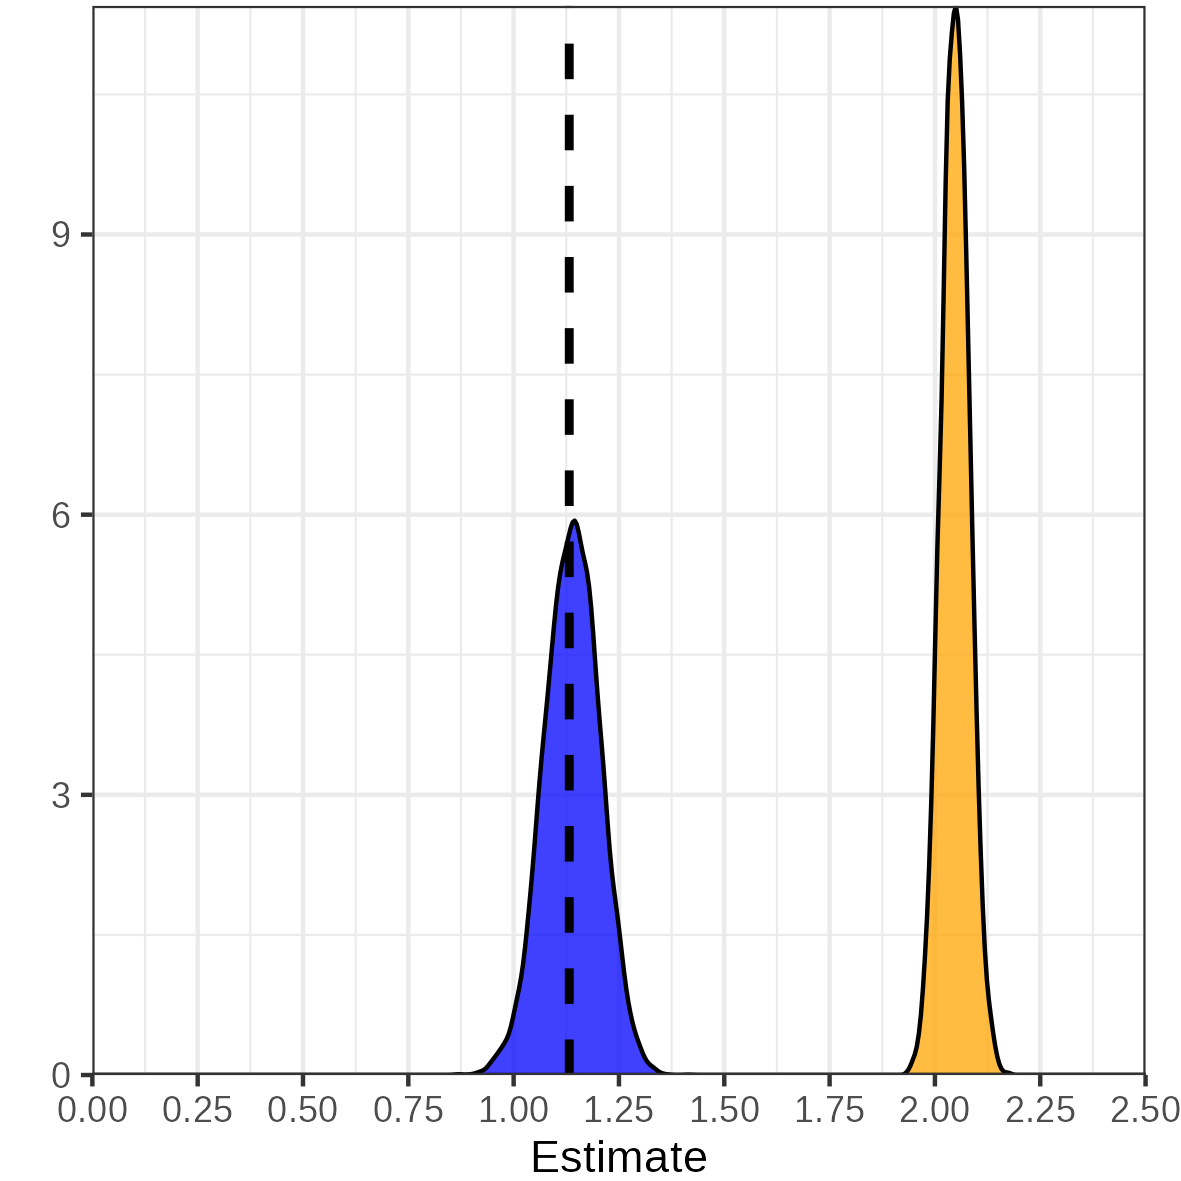
\includegraphics[width=\textwidth]{
            ../programs/simulations/sim-output/heckit-indirect-dist.png}
    \end{subfigure}
    \label{fig:cm-heckit-dist}
    \justify
    \footnotesize    
    \textbf{Note:}
    These figures show the empirical density of point estimates, for 10,000 replications of the data generated from a Roy model (described in \autoref{sec:controlfun}).
    The black dashed line is the true value;
    orange is the distribution of conventional CM estimates,
    and blue estimates with a Heckman selection adjustment.
\end{figure}
